% \input{\pSections "sec-input.tex"}

\section{Preparing for Mercury MoM}

%%%   %%%   %%%   %%%
\subsection{\texttt{*.stl} $\Rightarrow$ \texttt{*.obj}}
\begin{frame}\frametitle{CAD file (\stl) to Mesh Structure File (\obj)}
Many Tools For Converting \stl \ to \obj
\begin{enumerate}
	\item \href{https://www.blender.org/}{Blender}
	\item \href{https://www.freecad.org/}{FreeCAD}
	\item \href{https://openscad.org/}{OpenSCAD}
	\item \href{https://www.solidworks.com/}{SolidWorks}
	\item \href{https://www.tinkercad.com/}{Tinkercad}
	\item \href{https://www.meshconvert.com/}{MeshConvert.com}
	\item \href{https://www.greentoken.de/onlineconv/}{Online 3D Model Converter}
	\item others
\end{enumerate}
\end{frame}

%%%   %%%   %%%   %%%
\subsection{Structure of \texttt{*.obj}}
\begin{frame}{Seeing the \texttt{*.obj} File}
    \centering
    \begin{tabular}{ccc}
        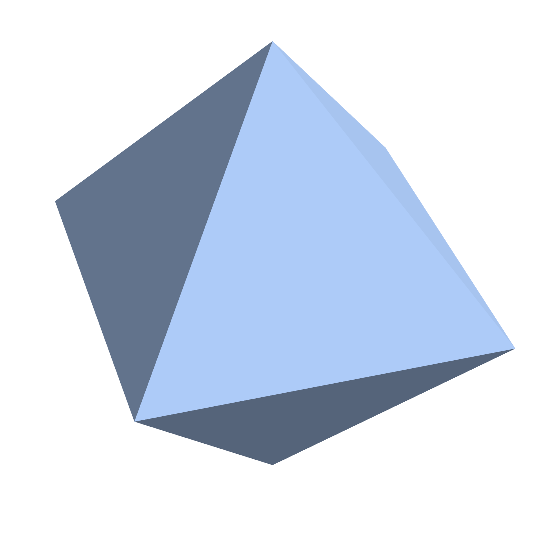
\includegraphics[width=0.3\textwidth]{\pLocalGraphics/spheres-0006.pdf} &
        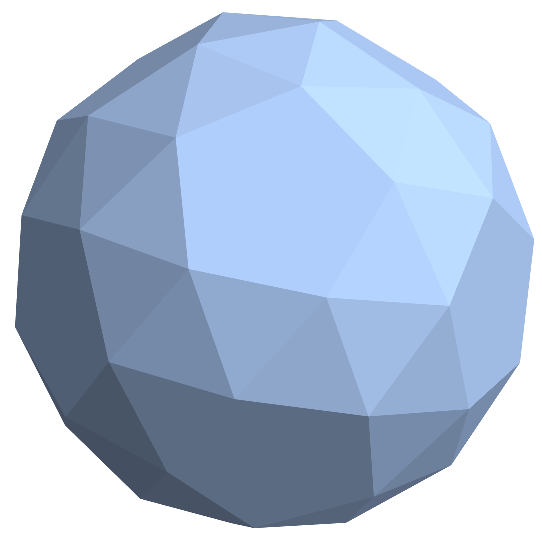
\includegraphics[width=0.3\textwidth]{\pLocalGraphics/spheres-0060.pdf} &
        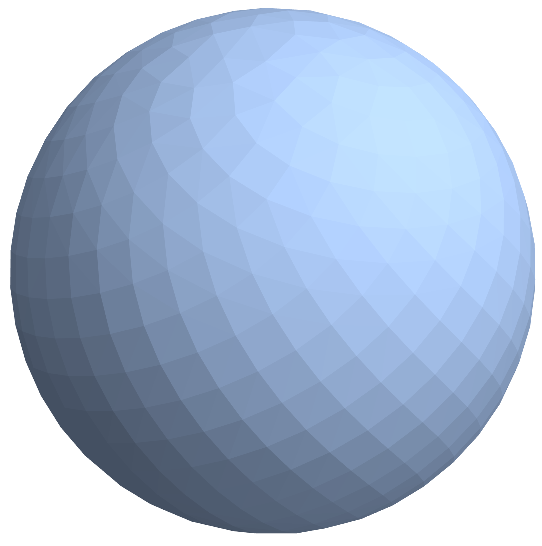
\includegraphics[width=0.3\textwidth]{\pLocalGraphics/spheres-0600.pdf} \\
        6 vertices & 60 vertices & 600 vertices \\
    \end{tabular}

    \vspace{0.5cm}
    \textbf{Decadal Improvement in Resolution:} \\Number of vertices increases $\times 10$
\end{frame}

%\begin{frame}[fragile]{Viewing the \texttt{sp-006.obj} File}
%    \lstset{style=terminal,
%    numbers=left,
%    numberstyle=\tiny\color{gray},
%    stepnumber=1,
%    numbersep=10pt
%}
%    \lstinputlisting{\pLocalData/sp-006.obj}
%\end{frame}

\lstdefinestyle{obj}{
    basicstyle=\ttfamily\listingFontSize,
    backgroundcolor=\color{black!5},
    frame=single,
    framerule=0.5pt,
    rulecolor=\color{black!50},
    xleftmargin=0.5cm,
    xrightmargin=0.5cm,
    breaklines=true,
    numbers=left, % Enable line numbers
    numberstyle=\tiny\color{gray},
    stepnumber=1,
    numbersep=10pt,
    numberbychapter=false % Prevent resetting line numbers
}

\begin{frame}[fragile]{\texttt{sp-006.obj}}
    \begin{columns}[T] % Top-aligned columns
        \column{0.48\textwidth}
        \lstset{style=obj} % Use the "obj" style
        \lstinputlisting[firstline=1, lastline=16]{\pLocalData/sp-006.obj} % Lines 1-16
        
        \column{0.48\textwidth}
        \lstset{style=obj} % Use the "obj" style
        \lstinputlisting[firstline=17, firstnumber=17]{\pLocalData/sp-006.obj} % Lines 17-end
    \end{columns}
\end{frame}

\newcounter{listnumber}

\begin{frame}{Components of the \texttt{*.obj}}
    \begin{enumerate}
        \item \textbf{Headers and Comments} (\#):
            \begin{itemize}
                \item Used for metadata or human-readable information.
                \item Example: \texttt{\# Created with Wolfram Language}.
            \end{itemize}

        \item \bl{Vertex Positions} (\texttt{v}):
            \begin{itemize}
                \item Specifies 3D coordinates for vertices.
                \item Example: \texttt{v 0 0 -1}.
            \end{itemize}

        \item \bl{Faces} (\texttt{f}):
            \begin{itemize}
                \item Defines polygons by referencing vertex indices.
                \item Example: \texttt{f 1/2/3}.
            \end{itemize}
    \end{enumerate}
        \setcounter{listnumber}{\value{enumi}}
\end{frame}

\begin{frame}{Components of the \texttt{*.obj}}
    \begin{enumerate}
         \setcounter{enumi}{\value{listnumber}}
        \item \textbf{Material Library Reference} (\texttt{mtllib}):
        %\item External \texttt{mtl} file that specifies \textbf{visual materials} 
      %for rendering (e.g., color, shading 
\includegraphics[width=0.05\textwidth]{\pLocalGraphics/palette.png} ).

        \begin{itemize}
        		\item External \mtl \ file that specifies \bl{visual materials} for rendering (e.g., color, shading) %
\includegraphics[width=0.05\textwidth]{\pLocalGraphics/palette.png}
        		\item Example: \texttt{sp-006.mtl}.
        		\item \textbf{Important Note}:  
              	This \mtl \ file is \rd{not related} to the \bl{electromagnetic materials} library in CAD models, which defines physical properties like permittivity, permeability, or conductivity.%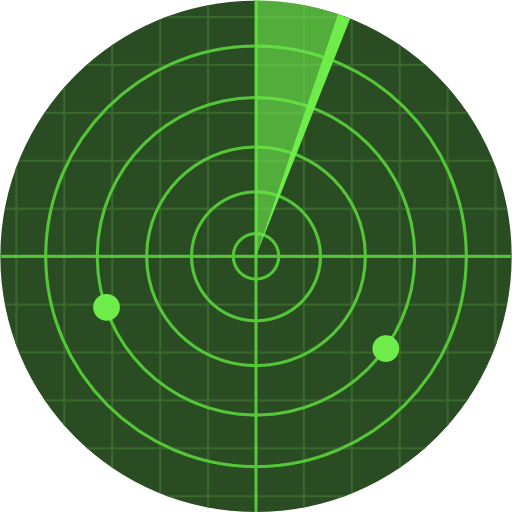
\includegraphics[width=0.05\textwidth]{\pLocalGraphics/radar.png}
    \end{itemize}
    \end{enumerate}
\end{frame}

%%%   %%%   %%%   %%%
\subsection{Structure of \texttt{*.facet}}

%%%   %%%   %%%   %%%
\subsection{Tools: Python}
\renewcommand{\listingFontSize}{\tiny} 
\begin{frame}[fragile,allowframebreaks]{Python Tool for \texttt{*.obj} to \texttt{*.facet}}
    \lstset{style=python} % Use the Python style
    \lstinputlisting{\pLocalCode/Obj2Facet_Python3.py}
\end{frame}

%%%   %%%   %%%   %%%
\subsection{Tools: Mathematica}
% nb: /Users/dantopa/Mathematica_files/nb/projects/hii-tsd/radar/obj/obj-02.nb
\renewcommand{\listingFontSize}{\tiny} 
\begin{frame}[fragile,allowframebreaks]{Mathematica Commands}
    \lstset{style=mathematica} % Use the Mathematica style
    
    \begin{lstlisting}
    (* Generate a mesh for a convex hull of points on a sphere *)
    mesh = ConvexHullMesh[SpherePoints[60]] // Region;

    (* Extract vertex coordinates from the mesh *)
    vlist = MeshCoordinates[mesh];

    (* Label each point in the mesh *)
    labeledPoints = MapIndexed[
        Text[Style[ToString[#2[[1]]], Bold, Black], #1] &, vlist
    ];
    \end{lstlisting}
\end{frame}

\endinput  %  ==  ==  ==  ==  ==  ==  ==  ==  ==
